\documentclass[11pt]{beamer}
\usetheme{Madrid}
\usepackage[utf8]{inputenc}
\usepackage{amsmath}
\usepackage{svg}

\usepackage{tikz-cd}

\author[\texttt{sebastiano.tronto@uni.lu}]{Sebastiano Tronto}
\title{Mathematical Software - Introduction}
\logo{
\includegraphics[scale=0.1]{img/unilu.jpg}} 
%\institute{University of Luxembourg} 

\date{2021-02-19} 

\begin{document}

\begin{frame}
  \titlepage
\end{frame}

\begin{frame}
  \tableofcontents
\end{frame}

\section{What?}
\begin{frame}{What}
  \begin{columns}
    \column{0.6\textwidth}
    \begin{itemize}
      \item {\bf Latex} for writing scientific text 
      \item {\bf Sage} for computations
    \end{itemize}

    \column{0.4\textwidth}
    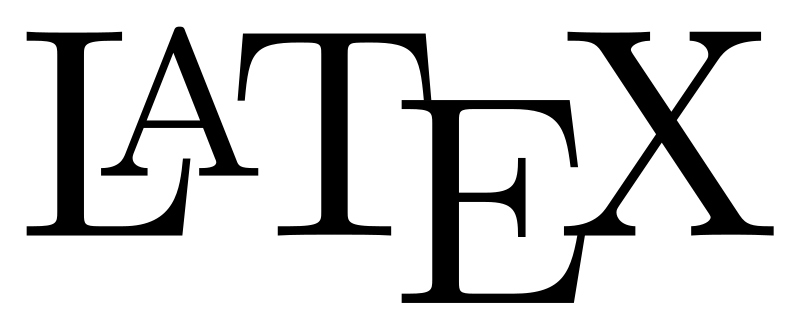
\includegraphics[scale=0.1]{img/latex.png}
    \vspace{0.5cm}

    \includesvg[scale=0.215]{img/sage}
  \end{columns}
\end{frame}

\subsection{Latex}
\begin{frame}{Latex}
  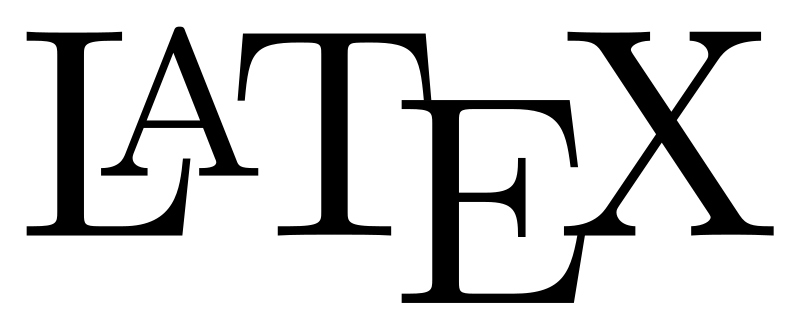
\includegraphics[scale=0.1]{img/latex.png}
  \begin{itemize}
    \item A typesetting system, has been around since the 1980s
    \item Currently the best way to write scientific texts (Math, Physics...)
    \item Can be used for lecture notes, homework, articles, books, graphics
          (with TikZ), this presentation...%, shopping list...
    \item ``What you get is what you \emph{mean}'', rather than what you
          \emph{see}
  \end{itemize}
\end{frame}

\begin{frame}[fragile]{Latex - Example}
  An equation like this:
  \begin{align*}
    e^x =& \sum_{n=0}^{\infty} \frac{x^n}{n!} \\
        =& 1 + x + \frac{x^2}{2} + \frac{x^3}{6} + \cdots
  \end{align*}
  is written in LaTeX as:
  \begin{verbatim}
    \begin{align*}
      e^x =& \sum_{n=0}^{\infty} \frac{x^n}{n!} \\
          =& 1 + x + \frac{x^2}{2} +
             \frac{x^3}{6} + \cdots
    \end{align*}
  \end{verbatim}
\end{frame}

\subsection{Sage}
\begin{frame}{Sage}
  \includesvg[scale=0.215]{img/sage}
  \begin{itemize}
    \item Free and open source Mathematical software
    \item Basically python with a lot of Math libraries
    \item Builds up on existing software such a Pari/GP, NumPy, R...
    \item Popular for Computational Algebra (Number Theory, Cryptography...)
  \end{itemize}
\end{frame}

\section{When?}
\begin{frame}{When}
  \begin{tabular}{r|c|c}
    %Date & Time & Topics \\
    %\hline
    February 19 & \texttt{14:00 - 17:30} & Introduction, LaTeX fundamentals  \\
    \hline
    March 12    & \texttt{14:00 - 17:30} & More advanced LaTeX topics        \\
    \hline
    March 26    & \texttt{14:00 - 17:30} & LaTeX: presentations, graphics    \\
    \hline
    April 2     & \texttt{14:00 - 17:30} & ??? (LaTeX or Sage)               \\
    \hline
    April 23    & \texttt{14:00 - 17:30} & Sage (???)                        \\
    \hline
    May 7       & \texttt{14:00 - {\bf 18:15}} & Sage (???)                  \\
    \hline
    May 21      & \texttt{14:00 - {\bf 18:15}} & Sage (???)
  \end{tabular}
\end{frame}

\section{How?}
\begin{frame}{How}
  \begin{itemize}
    \item \textbf{Remote teaching} at least until April 2 included (probably
          always).
    \item \textbf{Learn by doing} graded homework (4-5 assignments), non-graded
          exercises, free practice. No final exam.
  \end{itemize}
\end{frame}

\end{document}

